\documentclass{article}
\usepackage{geometry}
\usepackage[portuguese]{babel}
\usepackage[utf8]{inputenc}

\usepackage{graphicx}
\usepackage{caption}
\usepackage{float}

\usepackage{tikz}
\usepackage{amsmath}

\title{Resolução do Teste 2 de Tecnologias no Ensino da Matemática I}

\author{Carlos Frias}

\begin{document}

\maketitle

\begin{enumerate}
    \item \hfil
    \item Seja $T=\left(t_{ij}\right)_{1\leq i,j \leq n}$ uma matriz triangular inferior, que satisfaz $t_{ij}=0$, $i<j$, e é regular, ou seja $t_{ij}\neq0$, $i=1\left(1\right)n$. 
    Seja $T^{-1}$ a sua inversa dada por colunas, $T^{-1}=\left(z_1 \ldots z_n\right)$, onde $z_k={\left(0, \ldots, 0, z_{kk}, \ldots, z_{nk}\right)}^T$.
    Seja $I$ a matriz identidade também dada por colunas, $I=\left(e_1 \ldots e_k \ldots e_n\right)$, onde $e_k$ é o k-ésimo vector de base canónica. 
    Então, por definição de matriz inversa, sabemos que

    \begin{center}
        $TT^{-1}=I\Leftrightarrow Tz_k=e_k$, $k=1\left(1\right)n$ .
    \end{center}

    Explicitando as últimas igualdades, obtemos
    
    %Aqui as matrizes tenho que pesquisar um pouco mais para ver como fazer do jeito que tem que ficar
    \begin{equation}
        \begin{pmatrix}
            1 & 2 & 3\\
            a & b & c
        \end{pmatrix}
        \label{eq1}
    \end{equation}

    Efetuando as a multiplicação matricial em (\ref{eq1}), deduzimos as seguintes formulas para as componentes do vetor $z_k$
    
    \begin{center}
        $f(x)=\left\{
            \begin{array}{ll}
                \displaystyle z_{kk}=\frac{1}{t_{kk}}\\
                \displaystyle  \\
                \displaystyle z_{ik}=-\frac{1}{t_{ii}}\left(\sum_{j=k}^{i-1} t_{ij} z_{jk}\right),~i=k+1\left(1\right)n
            \end{array}\right.$
    \end{center}

    \item  \hfil
    
    \begin{figure}[H]
        \centering
        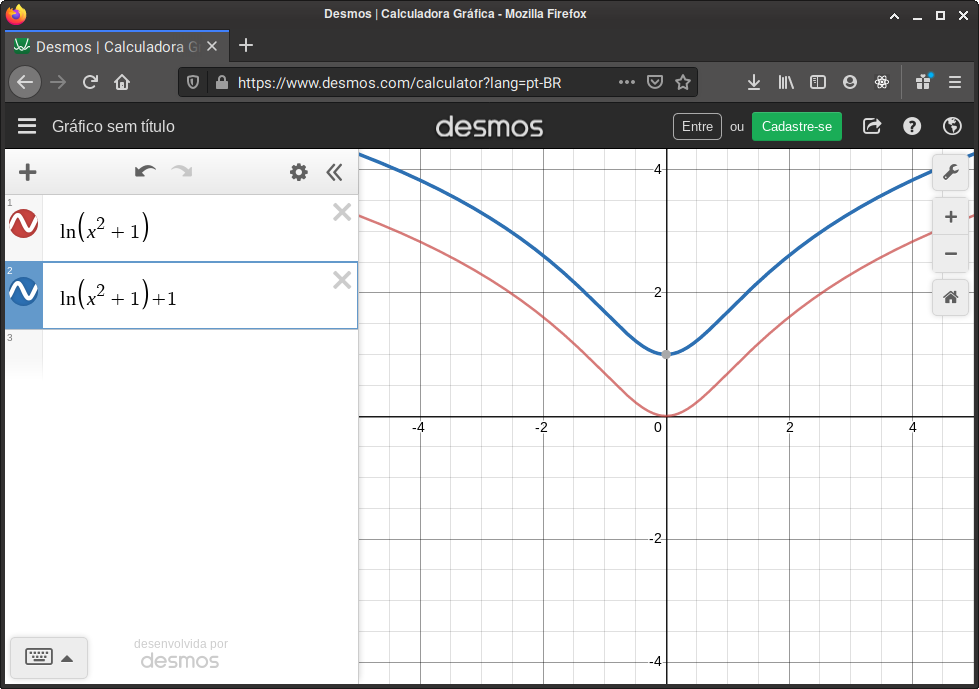
\includegraphics[width=\textwidth,keepaspectratio]{grafs.png}
        \caption{Gráfico feito no desmos}
    \end{figure}

    \begin{figure}[H]
        \centering
        \begin{tikzpicture}
            \draw[->,>=latex] (-4,0)--(4,0)node[below]{$x$};
            \draw[->,>=latex] (0,-1)--(0,4)node[left]{$y$};

            \draw[domain=-4:4, thick, blue, smooth, samples=50] plot (\x,{ln(\x*\x+1)}) node[above]{$f$};
            \draw[domain=-4:4, thick, red, smooth, samples=50] plot (\x,{1+ln(\x*\x+1)}) node[above]{$g$};
        \end{tikzpicture}
        \caption{Gráfico feito em TikZ}
    \end{figure}

    \item \textbf{Teorema 0.1.} A área da região do plano definida por $S\leq\tau\left(t\right)$, $t\in\left[a,b\right]$, 
    onde $\tau\left(t\right)$ é uma função contínua, não negativa e $b-a\leq2\pi$ é dada por 

    \begin{center}
        $\int_a^b \dfrac{\tau\left(t\right)^2}{2} dt$.
    \end{center}

    \textit{Demonstração.} Trivial!

    O teorema 0.1 aplica-se a curvas em coordenadas polares.

    \item
\end{enumerate}

\end{document}
